
\chapter{Testowanie}
\section{Frontend}
Testy w części frondendowej aplikacji wykonywane są przy pomocy platformy programistycznej Jest. W projekcie można wyróżnić podział na dwa typy testów. Pierwszym typem są testy spójności magazynu Vuex. Przykładowym testem tego typu jest test przypisanie tokenu JWT~(zob.~listing~\ref{lst:vuextest}). Celem testu jest sprawdzenie, czy funkcje odpowiadające za zapisywanie i odczytywanie danych zostały poprawnie zdefiniowane.
\begin{lstlisting}[caption=Test spójności magazynu Vuex,label={lst:vuextest}] 
describe('mutations', () => {
  test('setToken', () => {
    const token = "exampletoken"
    const state = {
      token: ""
    }
    store.commit('SET_TOKEN', { token })
    expect(store.getters.getToken.token).toBe(token)
  })
\end{lstlisting}

Drugim typem testów są testy interfejsu użytkownika. Przykładem takiego testu jest test przycisku, który odpowiada za zwiększanie liczby prowadzonych przez nauczyciela przedmiotów~(zob.~listing~\ref{lst:uitest}). Celem testu jest sprawdzenie, czy akcja wykonana przez użytkownika, w tym przypadku symulowana, skutkuje odpowiednią zmianą zmiennych w kodzie aplikacji. 
\begin{lstlisting}[caption=Test interfejsu użytkownika,label={lst:uitest}] 
describe('userInput', () => {
  test('addSubject', async () => {
    const wrapper = mount(Step2)
    const button = wrapper.find('addSubjectButton')

    expect(subjectNumber).toBe(0)
    await button.trigger('click')
    expect(subjectNumber).toBe(1)
})})
\end{lstlisting}
\section{Backend}
\subsection{Testowanie manualne}

Część backendowa, testowana była w dużym stopniu manualnie. Głównym narzędziem była aplikacja Postman. Przykładowe zapytanie wraz z odpowiedzią pokazano na rysunku ~\ref{rys:postman}.

\begin{figure}[H]
	\centering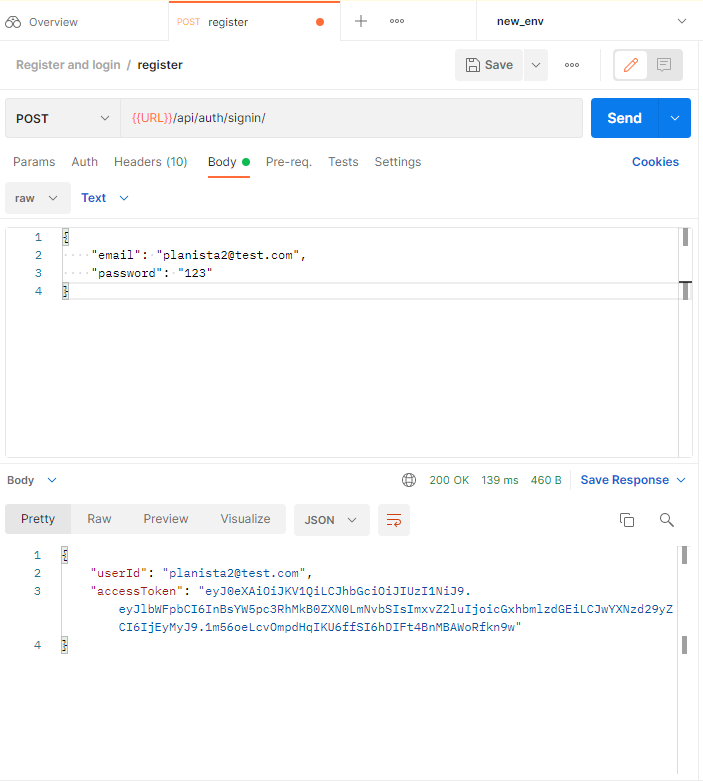
\includegraphics[width=\textwidth]{figures/postman1}
	\caption{Przykładowe zapytanie oraz odpowiedź w Postman}\label{rys:postman}
\end{figure}

Na zaawansowanych etapach implementacji, testy wykonywane były również z pomocą aplikacji frontendowej, dzięki czemu można była na bieżąco weryfikować integrację.

\subsection{Testy automatyczne}
Testami automatycznymi objęte zostały widoki oraz adresy URL. Do testowania widoków, wykorzystywane są testy integracyjne, natomiast do adresów testy jednostkowe. W obu przypadkach wykorzystywane są gotowe rozwiązania zaimplementowane w Django. Testy jednostkowe, sprawdzające poprawność implementacji adresów internetowych, sprawdzają czy podczas wysłania zapytania na dany adres, wywoływana jest opowiednia funkcja. Przykład implementacji takiego testu na listingu ~\ref{lst:TestJednostkowyBackend}.

\begin{lstlisting}[language=Python, caption=Implementacja przykładowego testu jednostkowego, label={lst:TestJednostkowyBackend}]
	class TestUrls(SimpleTestCase):
	
		def test_add_user(self):
			url = reverse('user')
			self.assertEquals(resolve(url).func, add_user)
\end{lstlisting}

Natomiast testy integracyjne, odpowiadające za widoki, mają za zadanie sprawdzić czy widok zwrócił odpowiednią odpowiedź HTPP. Przykład takiego testu na listingu ~\ref{lst:TestIntegracyjnyBackend}.

\begin{lstlisting}[language=Python, caption=Implementacja przykładowego testu integracyjnego, label={lst:TestIntegracyjnyBackend}]
	class TestViews(TestCase):
	
		def test_add_user_POST(self):
	
			email = 'test1@test2@.com'
			client = Client()
			url = reverse('user')
			
			Planners.objects.create(
			planneremail = email,
			login = 'test',
			password = 'test'
			)
			
			response = client.post(url, {
				'Sukces': 'Pomyslnie dodano uzytkownika'
			})
			
			self.assertEquals(response.status_code, 200)
\end{lstlisting}


\section{Algorytm}
	\subsection{Testy manualne}
	Testy manualne algorytmu przeprowadzane były przy pomocy przykładowych danych pierwotnie przygotowanych przez grupę inżynierską oraz ostatecznie uzyskanych z przykładowej istniejącej szkoły średniej. Dzięki wykorzystaniu danych z prawdziwej szkoły powstałą możliwość porównania planów generowanych przez algorytm z planem stworzonym przez wyszkolonego planistę w szkole średniej.	Dzięki temu możliwe było zwrócenie uwagi na niedoskonałości planu wygenerowanego względem tego stworzonego przez planistę oraz wyeliminowanie ich. Dzięki takim testom manualnym plany generowane przez algorytm udało się doprowadzić do stanu co najmniej bliskiego w stosunku do planu stworzonego przez wyszkolonego planistę.
	
	\subsection{Testy automatyczne}	
	Automatyczne testy jednostkowe algorytmu odbywają się przy pomocy biblioteki \textit{pytest}. Dzięki tej bibliotece testy napisane w języku python można wywóływać przy pomocy jednej komendy. Przykładowym testem jednostkowym jest sprawdzenie czy dane uzyskane z backend'u zostały prawidłowo przetworzone przez algorytm w celu ułatwienia wykonywania na nich różnych operacji. Poniższy test sprawdza, czy ilość danych przygotowanych dla Algorytmu zgadza się z ilością otrzymanych danych. (zob. listing 8.5)
	\newpage
	\begin{lstlisting}[language=Python, caption=Implementacja przykładowego testu jednostkowego sprawdzającego spójność danych, label={lst:TestJednostkowy}]
	def test_data_structures(groups_data=GROUP_OLD, teachers_data=TEACHERS_OLD, classrooms_data=CLASSES_OLD):
    school = School(groups_data, teachers_data, classrooms_data)
    assert len(school.groups) == len(groups_data), "Groups copied incorrectly to dict of class Group"
    assert len(school.classrooms) == len(classrooms_data), "Classrooms copied incorrectly to dict of class Classroom"
    assert len(school.teachers) == len(teachers_data), "Teachers copied incorrectly to dict of class Teacher"
\end{lstlisting}
	
	Kolejnym przykładem automatycznego testu jednostkowego jest sprawdzenie samego procesu ewolucji. Ocena gotowego najlepszego planu z pierwszego pokolenia jest zapisywana. Następnie przeprowadzony zostaje proces ewolucji. Ocena najlepszego planu uzyskanego z ostatniego pokolenia jest zapisywana. Podczas testu sprawdzane jest czy ocena uzyskana przez plan po procesie ewolucji jest lepsza, niż planu przed rozpoczęciem ewolucji. (zob. listing 8.6)
	
	\begin{lstlisting}[language=Python, caption=Implementacja przykładowego testu jednostkowego sprawdzającego proces ewolucji, label={lst:TestJednostkowy}]
	def test_evolution(groups_data=GROUP_OLD, teachers_data=TEACHERS_OLD, classrooms_data=CLASSES_OLD):
    population_size = 10
    num_of_generations = 100
    num_of_mutations = 20

    population = Population(groups_data=groups_data, teachers_data=teachers_data, classrooms_data=classrooms_data)
    population.new_population(number_of_instances=population_size)
    before_evolution = population.get_best_specimen().evaluation
    population.evolute(num_of_generations, num_of_mutations)
    after_evolution = population.get_best_specimen().evaluation

    assert before_evolution < after_evolution, "Before evaluation is not smaller than after evaluation"
    print("Evaluation before evolution is smaller than after evolution")
\end{lstlisting}
	
	 

